\documentclass[11pt, oneside]{amsart}   	% use "amsart" instead of "article" for AMSLaTeX format
\usepackage{geometry}                		% See geometry.pdf to learn the layout options. There are lots.
\geometry{a4paper}                   		% ... or a4paper or a5paper or ... 
\usepackage{graphicx}				% Use pdf, png, jpg, or eps with pdflatex; use eps in DVI mode
\usepackage{amssymb}
\usepackage{amsmath}
\usepackage{subfig}
\usepackage{courier}
\newcommand{\us}{\textunderscore}
\usepackage[round]{natbib}
\usepackage{hyperref}
\usepackage{fullpage}
\usepackage{float}
\floatstyle{plaintop}
\restylefloat{table}

\title{COVID-19 Individual-Based Model with Instantaneous Contract Tracing}
\author{Rob Hinch, Will Probert, Anel Nurtay, Christophe Fraser}

\begin{document}
\maketitle

\section{Overview}
COVID19-IBM is an individual-based model (IBM) for simulating an outbreak of COVID-19 in a city and to analyse the effect of both passive and active intervention strategies.
The model includes demographic data, which control both the dynamics of the interactions of individuals as well as disease outcomes.
Within the model, the virus (SARS-CoV-2) is spread via interactions between individuals.  Interactions can be remembered in the model to facilitate contact-tracing.
Intervention strategies such as self-quarantining, testing and contact-tracing can then be analysed.

\section{Demographics}

Demographics of the modelled population are based upon UK-wide data for 2018 from the Office of National Statistics (ONS). 
Three age categories are modelled: children (0-17 years), adults (18-64 years) and the elderly (65+).
Every individual is part of household which forms an important part of each person's daily interactions.
Data on household size is from the ONS.

\begin{table}[!htbp]
\centering
\begin{tabular}{ |p{3cm}|p{7cm}|p{1.2cm}|  }
 \hline
 \multicolumn{3}{|c|}{Demographic Parameters} \\
 \hline
 Name   & Description & Value \\
 \hline
 \hline 
 \texttt{n\us total}    & Total population simulated  & 100,000  \\
\hline
\texttt{uk\us pop\us 0\us 17}    & UK population 0-17 years old  (millions)  & 14.05 \\
\texttt{uk\us pop\us 18\us 64}  & UK population 18-64 years old  (millions)  & 40.22 \\
\texttt{uk\us pop\us 65}        & UK population 65+ years old (millions)       & 10.04 \\
 \hline 
\texttt{uk\us house\us1} & UK households with 1 person (thousands) & 8,198 \\
\texttt{uk\us house\us2} & UK households with 2 person (thousands) & 9,609 \\
\texttt{uk\us house\us3} & UK households with 3 person (thousands) & 4,287 \\
\texttt{uk\us house\us4} & UK households with 4 person (thousands) & 3,881 \\
\texttt{uk\us house\us5} & UK households with 5 person (thousands) & 1,254 \\
\texttt{uk\us house\us6} & UK households with 6 person (thousands) & 596 \\
 \hline
\end{tabular}
\end{table}

\section{Interaction Network}

Interactions between individuals are modelled via membership of numerous networks which represent people's daily interactions.
An individual's membership to different networks leads to age-group assortativity in the interactions.
Previous studies of social contacts for infectious disease modelling have estimated the mean number of interactions that individual's have, stratified by age group~\citep{mossong2008social}.

Mean interactions by age-group are estimated by aggregating this data.  We use the term "interactions" between individuals to mean possible contact that can spread disease.  We use the term "connections" between individuals as a superset of possible "interactions".  The modelled networks represent all the connections between individuals.  

\medskip \medskip
\begin{table}[!htbp]
\centering
\begin{tabular}{ |p{5cm}|p{1.5cm}|  }
 \hline
 \multicolumn{2}{|c|}{Mean daily interactions} \\
 \hline
Age group  & Value \\
 \hline
 \hline 
Children (0-17 years) & 15 \\
Adults (18-64 years) & 13 \\
Elderly (65 years+) & 7 \\
 \hline
\end{tabular}
\end{table}
\medskip \medskip

The model contains 3 types of networks: households, work-places (for children this would represent school) and random daily interactions.  Each simulated individual is a member of one of each type of network.  

\subsection{Household Network}
Each individual is assigned to live in a single household.  The proportion of people in each household is informed using UK household data (see Demographics section).
Each day every person has an interaction with everybody within their household.
Elderly people are assumed to live in either a 1 or 2 person household with other elderly people, with the ratio of elderly 1 and 2 person households being the same as the general population.
Children are assumed to live in household with two adults (so they can only live in 3/4/5/6 person households). 
The proportion of 3/4/5/6 person-households with children is the same as the those with adults only.

\subsection{Work-place Network}
Each individual is part of a single work-place network.
Work-place networks are modelled as Watts-Strogatz small-world networks (Watts and Strogatz, 1998).
A work-place network is modelled for each age group, with the network for children and elderly  containing a small proportion of adults (i.e.\ teachers and carers).
When constructing work-place networks individuals are randomly sorted, to ensure there is no unanticipated relationship between the household interactions and the local interactions on the small-world network.
Each day every person interacts with a random subset of their connections on their work-place network.

\begin{table}[!htbp]
\centering
\begin{tabular}{ |p{6.3cm}|p{6.8cm}|p{1cm}|  }
 \hline
 \multicolumn{3}{|c|}{Work-place Network Parameters} \\
 \hline
 Name   & Description & Value \\
 \hline
 \hline 
\texttt{mean\us work\us interaction\us child}    & Mean number of connections for children & 10 \\
\texttt{mean\us work\us interaction\us adult}  & Mean number of connections for adults & 7 \\
\texttt{mean\us work\us interaction\us elderly} & Mean number of connections for elderly & 3 \\
\hline
\texttt{child\us network\us adults} & Fraction of adults in child network & 0.2 \\
\texttt{elderly\us network\us adults} & Fraction of adults in elderly network & 0.2 \\
\hline
\texttt{daily\us fraction\us work} & Fraction of daily work connections made & 0.5 \\
\texttt{prob\us network\us rewire}$^*$ & Probability of rewiring a connection in the Watts-Stogatz small-world network & 0.1 \\ 
 \hline
\end{tabular}
\end{table}

The difference in the number of interactions for each age group is due to the overall number of daily interactions that each group have.  

\subsection{Random Network}

In addition to the structured networks of households and work-places, within which recurring daily interactions may occur, a number of random interactions are also included.  
Random interactions are drawn each day and are independent of the previous day's connections.
The number of random connections an individual makes is the same each day (without interventions) and is drawn at the start of the simulation from a negative-binomial distribution.
This variation in the number of interactions introduces "super-spreaders" into the network who have a much larger numbers of interactions than the average individual.

\begin{table}[!htbp]
\centering
\begin{tabular}{ |p{7.2cm}|p{6.8cm}|p{0.9cm}|  }
 \hline
 \multicolumn{3}{|c|}{Random Network Parameters} \\
 \hline
 Name   & Description & Value \\
 \hline
 \hline 
\texttt{mean\us random\us interaction\us child}    & Mean number of connections for children & 2 \\
\texttt{mean\us random\us interaction\us adult}    & Mean number of connections for adults & 4 \\
\texttt{mean\us random\us interaction\us elderly} & Mean number of connections for elderly & 3 \\
\hline
\texttt{sd\us random\us interaction\us child}$^*$  & s.d.\ number of connections for children & 2 \\
\texttt{sd\us random\us interaction\us adult}$^*$ & s.d.\ number of connections for adults & 4 \\
\texttt{sd\us random\us interaction\us elderly}$^*$ & s.d.\ number of connections for elderly & 3 \\
 \hline
\end{tabular}
\end{table}

The mean numbers of random connections were chosen so that the total number of daily interactions matched that from the social interaction studies. 
The split between work and random interactions was chosen to be lower in children. 
Each day a list is made which contains all individuals who make random interactions and each person is repeated by the number of interactions they make.
This list is then randomly shuffled and interactions are made between adjacent pairs on the shuffled list.

\section{Infection Dynamics}

The disease is spread by interactions between infected and susceptible individuals.
The probability of transmission is determined by the infection status of the infected individual and the age of the susceptible.
Note that the type of interactions (i.e.\ household, work or random) or the length of the interaction (currently not modelled) is not used in deciding the likelihood of transmission.
From early studies of SARS-CoV-2~\citep{lai2020severe,guan2020clinical} and analyses of other epidemics~\citep{chan2003sars,meltzer2004multiple}, we know that immediately after becoming infected an individual is not infectious.
The level of infectiousness increases with time and peaks typically 5-7 days after the initial infection before decreasing.  
Following~\citep{ferretti2020quantifying}, we model infectiousness since time of infection using a gamma function, and the infectiousness on day $t$ after infection is calculated by integrating the gamma function from $t-1$ to $t$.

It has been observed that some people who are infected with SARS-CoV-2 remain completely asymptomatic~\citep{bai2020presumed}, and we assume that these people are less infectious then those who go on to develop symptoms. 
Note, there is a difference between somebody who is asymptomatic (\emph{i.e.} who will never go on and develop symptoms), as opposed to somebody who is pre-symptomatic (\emph{i.e.} who will go on and develop symptoms at some point). 
The term ``pre-symptomatic'' is used to describe people who are infectious while not having symptoms. 
In study conducted on SARS-CoV-2 positive patients from Singapore~\citep{young2020epidemiologic}, infected individuals, whose symptoms had had already faded, had detectable respiratory shedding of the virus. 
While modelling, we combine the pre- and post-symptomatic infectious individuals under the common category and call them, for simplicity, pre-symptomatic. 
The pre-symptomatic infected individuals are assumed to have the infectiousness level that is similar to the one of symptomatic infected individuals~\citep{young2020epidemiologic,rothe2020transmission}.

Heterogeneity in susceptibility also plays a factor in transmission. 
Data from the Chinese CDC suggest that the children are far less susceptible to infection than adults, and that the elderly are more susceptible than adults~\citep{chinavital},.  
The model accounts for differences in susceptibility by a simple multiplicative factor based upon the age group of the susceptible individual.

Combining all effects, we model the rate at which the virus being transmitted in a single interaction by
\begin{equation}
\lambda(t,a_s,b) = \frac{R s_{a_s}A_b}{ \bar I_{a_s}} \int_{t-1}^t f_{\Gamma}(u; \mu_i,\sigma_i^2) {\rm d}u,
\end{equation}
where $f_{\Gamma}(u; \mu_i,\sigma_i^2)$ is the p.d.f.\ of a gamma distribution with mean $\mu$ and variance $\sigma^2$; $t$ is the number of days since the infector become infected; $a_s$ is the age group of the susceptible; $b$ is an indicator of whether the infected individual is asymptomatic; the other terms listed in the Infectious Parameters table  (see Table~\ref{table_infectious_parameters}).
The rate of virus transmission is converted to a probability of transmission  ($P(t,a_s,b)$) using the formula
\begin{equation}
P(t,a_s,b) = 1 - e^{-\lambda(t,a_s,b)}.
\end{equation}
The epidemic is seeded by randomly infecting a small number of individuals at the start of the infection.  Seed cases are assumed to have been infected immediately before the simulation starts.

\begin{table}
\centering
\resizebox{\textwidth}{!}{
\begin{tabular}{|l|l|l|l|}
 \hline
 \multicolumn{4}{|c|}{Infection Parameters} \\
 \hline
 Symbol & Name   & Description & Value \\
 \hline
 \hline 
$R$ & \texttt{infectious\us rate} & mean number of people infected by each infected person & $2.5^{\times}$ \\
$A_{\rm sym}$ &  - & relative infectious rate of symptomatic & 1 \\
$A_{\rm asym}$ & \texttt{asymptomatic\us infectious\us factor}& relative infectious rate of asymptomatic & 0.25 \\
 \hline
 $\mu_i$ &  \texttt{mean\us infectious\us period} & time of peak infectiousness (i.e.\ the mean of the gamma p.d.f.) & $6^{\times}$  days\\
 $\sigma_i$ &  \texttt{sd\us infectious\us period} & width of infectiousness curve (i.e.\ the s.d.\ of the gamma p.d.f.) & $2^{\times}$ days\\
 \hline
 $s_{\rm child}$   &  \texttt{relative\us susceptibility\us child} & relative susceptibility of child to adult & $0.1^*$ \\
 $s_{\rm adult}$   &   - &  - & $1^*$\\
 $s_{\rm elderly}$ &  \texttt{relative\us susceptibility\us elderly} & relative susceptibility of elderly to adult & $1.7^*$ \\
 \hline
  -&  \texttt{n\us seed\us infection} & number of individual randomly infected at start of simulation & 10 \\
 \hline
\end{tabular}}
\caption{Description of infection parameters and their values. Infectious rate and corresponding infectiousness parameters$^{\times}$ were obtained in Ref.~\citep{ferretti2020quantifying}. Relative values\protect{$^*$} are derived from the study of 44,672 confirmed patients in China~\protect{\citep{chinavital}}.}
\label{table_infectious_parameters}
\end{table}

\section{Disease Dynamics}

Upon infection, an individual enters a disease progression cascade where the outcome and rates of progression are dependent upon age of the infected person (figure \ref{diseaseDynamics}).
The first split is that only a fraction of individual who will develop symptoms, where a fraction ($\phi_{\rm asym}$) remain asymptomatic.
Those who are asymptomatic are infectious (at a lower level, see Infection Dynamics section) and will move to a recovered state after a time ($\tau_{\rm a,rec}$) drawn from a gamma distribution.
Once an individual is recovered we assume that they have lifelong immunity and cannot be reinfected.

For individual who will develop symptoms, they start by being in the pre-symptomatic state, where, whilst they will be able to transmit the disease to others, they will not be showing any symptoms. 
This is important for modelling interventions because individuals in this state would not be able self-isolate unless they had been contact-traced (or there was a complete shutdown).
After a time ($\tau_{\rm sym}$) drawn from a gamma distribution, the individual develops symptoms, at which case interventions can be triggered such as self-isolation, testing and contact-tracing.
Whilst most individuals will only develop mild symptoms, a fraction ($\phi_{\rm hosp}({\rm age})$) will go on to require hospitalisation, where the probability of requiring hospital treatment is age-dependent.
Those individuals who do not require hospitalisation will recover after a time ($\tau_{\rm rec}$) drawn from a gamma distribution, whilst those who require hospital treatment enter after a time ($\tau_{\rm hosp}$) drawn from a Bernoulli distribution of either 1 or 2 days.
Once entering hospital, a number of interventions can take place. 
We assume that a clinical diagnosis can immediately decide whether the patient is a case so that contract-tracing can be commenced straight away.
Of those who enter a hospital, a fraction ($\phi_{\rm death}({\rm age})$) will die with the rest recovering. 
The time to death ($\tau_{\rm death}$) and recovery ($\tau_{\rm death}$) are both drawn from gamma distributions.

The disease state transitions are shown in (figure \ref{diseaseDynamics}) and the model parameters are in the table Disease Dynamics Parameters.

\begin{figure}
\centering
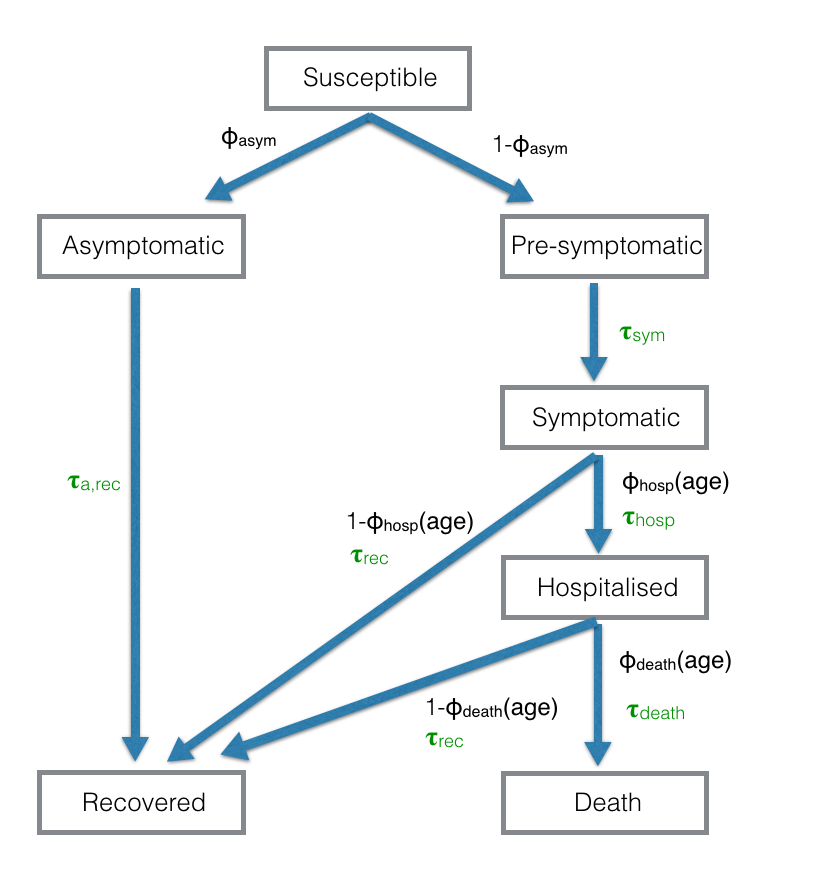
\includegraphics[width=.9\textwidth]{diseaseDynamics.png}
\caption{The disease status of an individual and the probability and time distribution of transitions. The $\phi_{\rm xxx}(\rm age)$ variables are the probability of transition to a particular state when there is a choice, where the probability depends upon the age of the individual.  The $\tau_{\rm xxx}$ are the gamma distributed variables of the time taken to make the transition.}
\label{diseaseDynamics}
\end{figure}

\begin{table}
\centering
\begin{tabular}{ |p{2.3cm}|p{6.4cm}|p{4cm}|p{1.4cm}|  }
 \hline
 \multicolumn{4}{|c|}{Disease Dynamics Parameters} \\
 \hline
 Symbol & Name  & Description & Value \\
 \hline
 \hline 
  $\phi _{\rm asym} $  &  \texttt{fraction\us asymptomatic} & fraction of infected who are asymptomatic & 0.2 \\
 \hline
 $\phi_{\rm hosp} ({\rm child } )$     &  \texttt{hospitalised\us fraction\us child}    & fraction of symptomatic children hospitalised & 0.15 \\
 $\phi_{\rm hosp} ({\rm adult } )$    &  \texttt{hospitalised\us fraction\us adult}    & fraction of symptomatic adults hospitalised & 0.15 \\
 $\phi_{\rm hosp} ({\rm elderly } )$ &  \texttt{hospitalised\us fraction\us elderly} & fraction of symptomatic elderly hospitalised & 0.25 \\
 \hline
 $\phi_{\rm death} ({\rm child } )$    &  \texttt{fatality\us fraction\us child}     & fraction of hospitalised children who die & 0.01 \\
 $\phi_{\rm death} ({\rm adult } )$    &  \texttt{fatality\us fraction\us adult}    & fraction of hospitalised adults who die & 0.04 \\
 $\phi_{\rm death} ({\rm elderly } )$ &  \texttt{fatality\us fraction\us elderly} & fraction of hospitalised elderly who die & 0.25 \\
 \hline
$\mu_{\rm sym} $       &  \texttt{mean\us time\us to\us symptoms} & mean time to symptoms & 5.5 days \\
$\sigma_{\rm sym} $  &  \texttt{sd\us time\us to\us symptoms}       & s.d.\ time to symptoms & 2.5 days \\
 \hline
$\mu_{\rm sym} $       &  \texttt{mean\us time\us to\us symptoms} & mean time to symptoms & 5.5 days \\
$\sigma_{\rm sym} $  &  \texttt{sd\us time\us to\us symptoms}       & s.d.\ time to symptoms & 2.5 days \\
 \hline
$\mu_{\rm hosp} $       &  \texttt{mean\us time\us to\us hospital}  & mean time to hospital after showing symptoms & 1.6 days \\
 \hline
$\mu_{\rm death} $       &  \texttt{mean\us time\us to\us death} & mean time to death once hospitalised & 12 days \\
$\sigma_{\rm death} $  &  \texttt{sd\us time\us to\us death}       & s.d.\ time to death once hospitalised & 5 days \\
 \hline
$\mu_{\rm rec} $       &  \texttt{mean\us time\us to\us recover} & mean time to recover after symptoms/hospital &  12 days \\
$\sigma_{\rm rec} $  &  \texttt{sd\us time\us to\us recover}       & s.d.\ time to recover after symptoms/hospital & 5 days \\
 \hline
$\mu_{\rm a,rec} $       &  \texttt{mean\us asymptomatic\us to\us recover} & mean time to recover after asymptomatic &  15 days \\
$\sigma_{\rm a,rec} $  &  \texttt{sd\us asymptomatic\us to\us recover}       & s.d.\ time to recover after asymptomatic & 5 days \\
 \hline
\end{tabular}
\end{table}

\section{Passive Interventions}

The model has the ability to model both passive and active interventions. 
Here we define an active intervention to be one involving testing or contact-tracing with all other interventions being classed as passive.
Interventions are designed to reduce the rate of transmission, however, have the side-effect of potentially quarantining significant numbers of people. 

\subsection{Hospitalisation} Upon hospitalisation, a patient immediately stops interacting with both their household and work-place networks. We also reduce the number of random interactions that they have. An aspect of the disease transmission that we are missing in the model are the interactions within hospitals. 

\subsection{Self-Isolation upon Symptoms} The next type of intervention we model is self-isolation upon flu-like symptoms. In addition to those infected by coronavirus, we infect a random a sample of the population each day with seasonal-flu which has similar symptoms. Upon experiencing symptoms, we put a fraction of patients in to self-quarantine immediately. 
Quarantine is modelled by not interacting with your work-place network and having a much reduced number of connections on your random network.
The length of quarantine is set to be 14 days, however, we model the fact that some people will dropout each day before the 14 days is reached.

\begin{table}
\centering
\resizebox{\textwidth}{!}{
\begin{tabular}{|l|l|l|l|}
 \hline
 \multicolumn{3}{|c|}{Passive Intervention Parameters} \\
 \hline
 Name   & Description & Value \\
 \hline
\hline
\texttt{self\us quarantine\us fraction} & proportion of people who self quarantine upon symptoms &  0.9 \\
\texttt{quarantine\us length\us self}  & maximum time of self-quarantined  & 14 days \\
\texttt{quarantine\us dropout\us self} & probability somebody drop out each day from self-quarantine & 0.01 \\
\texttt{quarantined\us daily\us interactions} & daily random interactions of a quarantined person &  0 \\
\texttt{hospitalised\us daily\us interactions} & daily random interactions of a hospitalised person &  0 \\
\texttt{seasonal\us flu\us rate} & daily probability of  seasonal flu &  0.0003  \\
 \hline
\end{tabular}}
\end{table}

\section{Active Interventions}
We define active interventions as those which involve either testing or actively tracing individuals who had contact with an infected person (i.e.\ contact-tracing).
There are 3 events in the model which can be the initial trigger for an active intervention.
Note, for contract-tracing to occur, one of these events must be the trigger.

\subsection{On flu-like symptoms} We have already described how some people will self-isolate when they display symptoms. 
However, there is also an intervention option to order a test for person who has flu-like symptoms. 

\subsection{On positive-test} When an individual has received a positive test, we can then immediately initiate contact-tracing if the person has the app.

\subsection{On hospitalisation} When an individual enters hospital with suspected COVID19 a test is ordered to confirm the diagnosis. In the model we give the intervention option of contact tracing to be commenced immediately upon a clinical diagnosis, without waiting for the test to confirm.

\medskip
The model has 2 types of active intervention, one is testing for coronavirus and the other is app-based contact-racing. 
These 2 interventions work together informing each other of the next steps.
\subsection{Testing} Currently the test for coronavirus is not sensitive immediately upon infection, which we model by only returning a positive test if the patient has been infected for 3 days when the test takes place. For individuals who already displaying symptoms this is not an issue since the symptoms normally only present after the test has become sensitive. However, when ordering tests while carrying out contact tracing, we need to take this in to account. Currently there are also delays in the testing procedure, both in taking a test and in getting the result for it. These test-delays are modelled which will then delay other interventions. Anyone receiving a positive test is quarantined for up to 14 days (with a random daily dropout) and there is the option to trigger app-based contract tracing.

\subsection{App-based Contact-Tracing} The second intervention we model is the app-based contract-tracing, which can initiate the quarantining of infected individuals prior to them ever showing symptoms. For infections with high levels of pre-symptomatic transmission this is vital to prevent epidemics. Contact-tracing can only originate from somebody with the app and can only trace others who have the app as well. Given that the whole population will not have the app, we randomly pick a fraction of the population to not have the app. Secondly, the app is likely to miss some interactions between individuals, even if both individuals have the app, so when contact-tracing we randomly drop a number of interactions. We then go through all the interactions of the individual for a number of days, and if the app recorded the interaction the contact can be asked to quarantine and/or be tested for coronavirus. There is also an option to recursively contact-trace where we automatically trace the contact of contacts who can also be asked to quarantine and/or be tested for coronavirus.

\begin{table}
\centering
\resizebox{\textwidth}{!}{\begin{tabular}{|l|l|l|}
 \hline
 \multicolumn{3}{|c|}{Active Intervention Parameters} \\
 \hline
 Name   & Description & Value \\
 \hline
 \hline
\texttt{app\us users\us fraction} & fraction of population with the app & 0.85 \\
\texttt{quarantine\us days} & the number of days prior contacts to contact & 5 days \\
\texttt{traceable\us interaction\us raction} & fraction of interactions that captured if both users have app & 0.8 \\
\texttt{tracing\us network\us depth} & depth of interaction network to contact (i.e.\ second-order contacts) & 2 \\
\hline
\hline
\texttt{quarantine\us on\us traced} & quarantine individuals who are traced & 1 \\
\texttt{test\us on\us traced}            & test individuals who have been contact-traced & 1 \\
\texttt{test\us on\us symptoms}      & test individuals who show symptoms and are quarantined & 1 \\
\texttt{tracing\us on\us clinical\us}  diagnosis & commence contact-tracing on a clinical diagnosis & 1 \\
\hline
\hline
\texttt{quarantine\us length\us traced}     & maximum time of quarantined if traced  & 14 days \\
\texttt{quarantine\us dropout\us traced}   & probability somebody drop out each day if traced  & 0.01 \\
\texttt{quarantine\us length\us positive}   & maximum time of quarantine if test positive & 14 days \\
\texttt{quarantine\us dropout\us positive} & probability somebody drop out each day if tested positve & 0.01 \\
\hline
\hline
\texttt{test\us insensitive\us period} & number of days following infection the test is insensitive & 3 days\\
\texttt{test\us order\us wait} & minimum number of days to wait to take a test  & 1 days \\
\texttt{test\us result\us wait} & number of days to wait for a test result & 1 days \\
 \hline 
\end{tabular}}
\end{table}

\section{Implementation Details}
This is a high-level description of how the model is implemented.
The model is coded in C but using an object-orientated pattern.
All required memory is pre-allocated at the start of the simulation for efficiency.

\subsection{Events} 
We use an event-based system to drive disease progression in individuals and interventions, where at each decision point we calculate when the next event will occur and add it to an event-list for that day.
For each type of event there is an \texttt{eventlist} structure, which contains an array of linked-lists for each day of the simulation.
We use doubly-linked lists to allow for efficient deletion as well as insertion of events.
Event-lists also keep track of the current and total number of events (defined as all entries today and in the past). 

\subsection{Individuals} 
Each person in the population is represented by an \texttt{individual} structure and the population is static.
The \texttt{individual} structure contains the following information:
\begin{enumerate}
\item Demographic - age, network membership
\item Interaction diary - list of all interactions over a period of days (note this is not just ones tracked by the app)
\item Disease - current status (i.e.\ symptomatic) and pointers to both current and future disease events
\item Quarantine - is the person currently quarantined and pointers to that event and the release event
\end{enumerate}

\subsection{Network Construction}
Each interaction network has an associated \texttt{network} structure which contains an array of edges.
Network structures can be static (i.e.\ household), static but down-sampled (i.e.\ work-place) or dynamically generated at each time step (i.e.\ random).
Network generation is modular and any network can be added to the model as long as it can be represented by an array of edges.
Once all the networks have been defined, we add each edge to the individuals interaction diary (which are single-linked lists as deletion is not required).

\subsection{Disease transmission}
The next step is to transmit the disease across today's interaction network, which is done as push from all infected people (by disease status).
For every infectious status, we pre-calculate the transmission rate for someone who has been infected for that length of time.
At each time-step, we go through all that interactions the infected person had for that day and calculate whether transmission has occurred.
Instead of randomly drawing whether transmission has occurred for each interaction, we allocate each individual a quantity of {\it hazard} (from an exponential distribution) at the start of the simulation.
Each interaction with an infected person reduces the persons {\it hazard} and when a person's {\it hazard} drops below 0 they become infected. 
This is mathematically equivalent to randomly drawing individual interactions, which can be seen by calculating the probability of  being infected by the $N^{\rm th}$ interaction  $P({\rm infected} \  N^{\rm th})$, after exposured to interactions with hazard-rates $\{ \lambda_1,..,\lambda_N \}$
\begin{align*}
P({\rm infected} \  N^{\rm th}) 
&= P_N \prod_{i=1}^{N-1} ( 1 - P_i) \\
&= \exp\left( -\sum_{i=1}^{N-1} \lambda_i \right) - \exp\left( -\sum_{i=1}^{N} \ \lambda_i\right) \\
&= P \left(  \sum_{i=1}^{N-1} \lambda_i  < T <  \sum_{i=1}^{N} \lambda_i \right)
\end{align*}
where $T$ is distributed exponentially with mean 1. 
The fact that different age groups have a different susceptibilities ($s_{a_s}$) is then modelled by allocating different amounts of initial {\\it hazard} to each group.
This improves computational efficiency so that is it not necessary to draw a random variable for each potential transmission event.

\renewcommand{\bibname}{References}
\bibliographystyle{abbrvnat}
\bibliography{lib} 
\end{document}  
